\section{ESMACS}

In the past, there has been a number of MMPBSA type calculations for DNA intercalator systems. A large majority of these studies only takes into account just a few (one to three) intercalators binding to the DNA, and does not compare to experimental studies. We obtained a correlation Pearson coefficient of $r_p=0.70$ across the 10 planar molecules for the 3 trajectory calculation.

\subsubsection{Convergence}

It is important to assess the sampling efficiency and converge of the predicted free energy values in order for the results to be reliable and reproducible.
First, the comparison in convergence between a single trajectory approach and an ensemble of trajectories is compared for the MMPBSA and NMODE analysis methods in the context of free energy calculations. As the improvement in ensemble methods was evident, we investigated the length of each replica, extending the simulations from the original 5 ns simulation to 20 ns for each of the 25 replicas. It was important to sample the system long enough to cover a large part of the phase space, but not to oversample in places where the methods is no longer valid, for example during a de-intercalation pathway.

\begin{figure}
  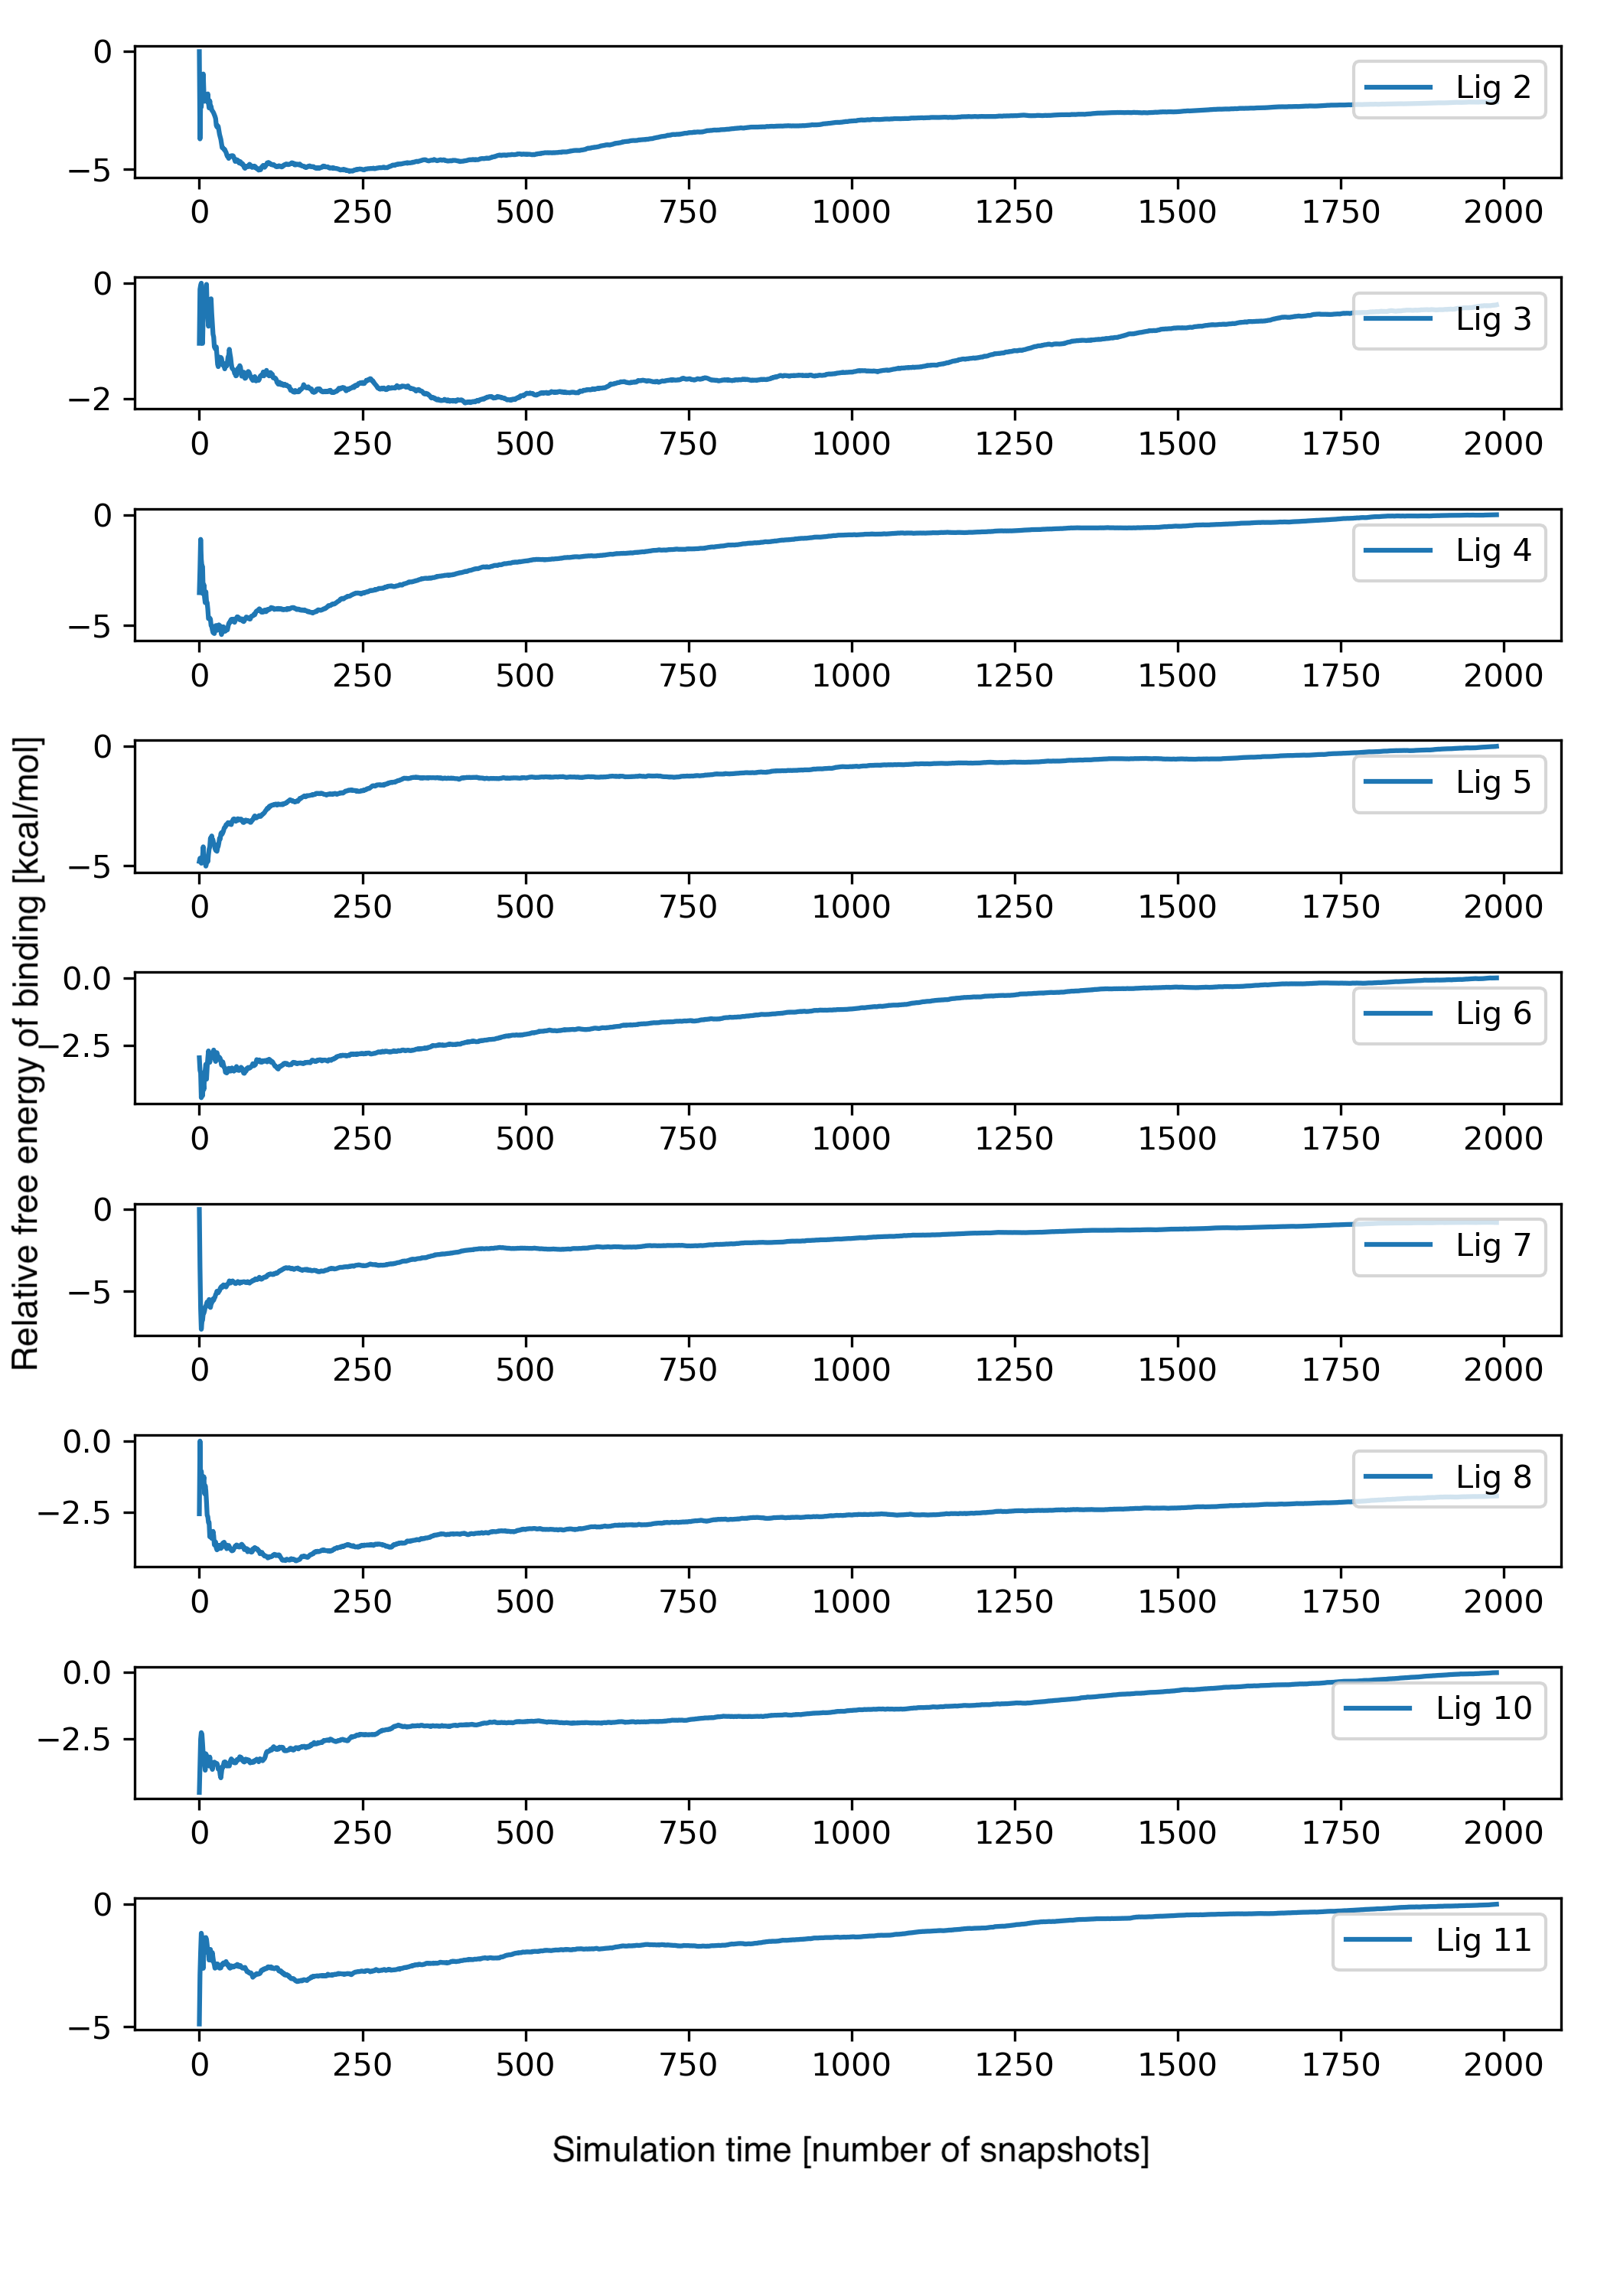
\includegraphics[width=\columnwidth]{mmpbsa_conv.png}
  \caption{Converge of the free energy for the 10 ligands investigated with the ESMACS method. The 4+16 ns equilibration and production run is used for all the intercalators to reach a converged result.}
  \label{fig:mmpbsa_conv}
\end{figure}

\subsubsection{Predicting the ranking}

The experimental free energy values are between -3.69 and -3.50 kcal/mol, making them hard to differentiate computationally. Approximate methods, like ESMACS, that are based on MMPBSA and NMODE for the free energy and entropy contribution, respectively do not have the resolution to differentiate experimental values at this scale. Nonetheless, correct error control and ensemble based calculations can give meaningful results relative to each other, i.e. ranking the intercalators based on their free energies will be comparable to experimental ranking.

We have run 1, 2 and 3 trajectory calculations and as seen in Figure~\ref{fig:mmpbsa} the correlation improves, with the 3 trajectory being the most accurate with a correlation coefficient of $r_p=0.70$. The small interval of the experimental values suggests that the intercalators are very closely binding to the DNA. 

The correlation achieved with ESMACS in this study suggests that one of the underlying forces (electrostatic, vdW, or internal energy) dominates the interaction gradient between the intercalators, and that signal is picked up by the MMPBSA calculation. Figure~\ref{fig:corrmat} shows the spread of the free energy values of the different components. Previous studies \cite{galindo2017computational} have shown that vdW interactions contribute most to the binding energy of the intercalators in absolute terms. However, the correlation of the different components to the total binding energy shows that the internal energy (the sum of bond, angle, and torsion terms) correlate with the total. This further supports our claim that the intercalation is an induced fit inside the two basepairs.

\begin{figure}
  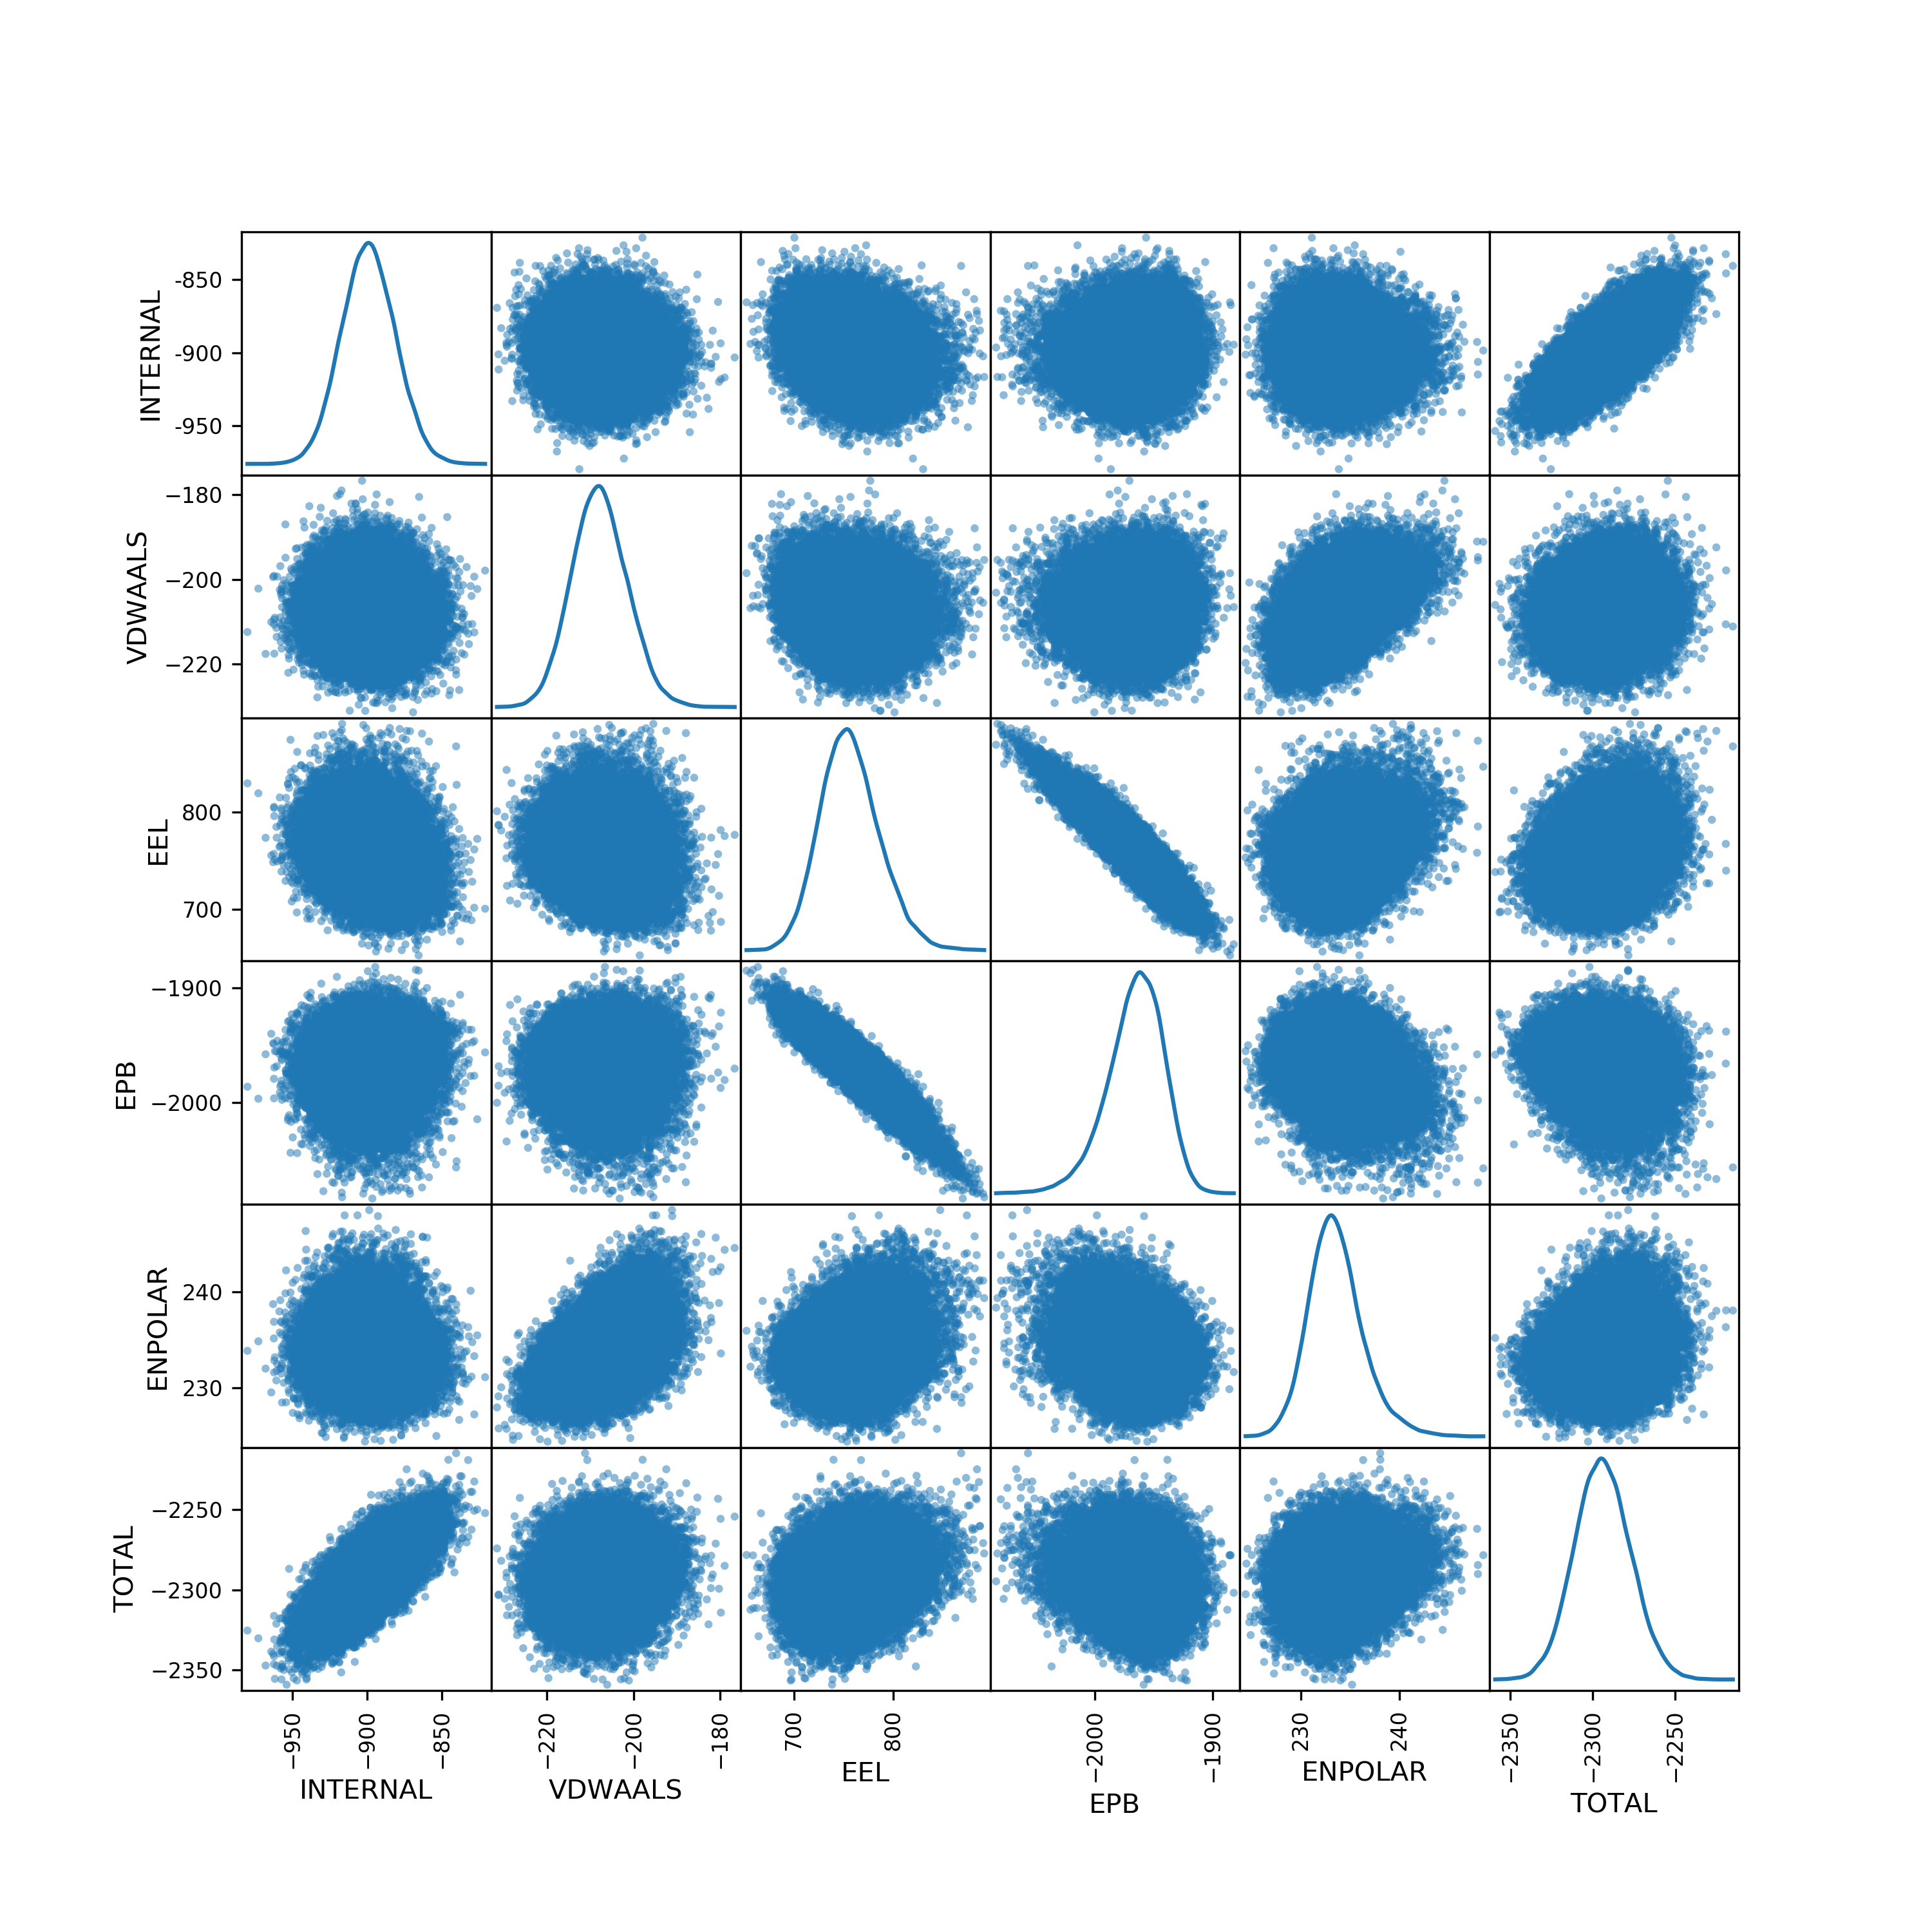
\includegraphics[width=\columnwidth]{components}
  \caption{A correlation plot of the different components contributing to the free energy in the MMPBSA study We compare the total to the different components to investigate which ones have some correlation.}
  \label{fig:corrmat}
\end{figure}

Each ESMACS calculation was run 25 times, the only difference being the random seed at the start of the simulation. 

Variations in the results from the different replica was used to evaluate the error on the predicted free energy. Figure~\ref{fig:bootstrap} shows the bootstrapped error as a function of the number of replicas. There is a levelling off at around 20 replicas, with 25 replicas showing consistently low error bars.

\begin{figure}
  \centering
  \begin{tikzpicture}
\begin{axis}[
  xlabel=Number of replicas,
  ylabel={Error (kcal/mol)},
  ]
  
  \addplot table {bootstrap.csv};
  
\end{axis}
\end{tikzpicture}
  \caption{Bootstrapped error as a function of replica size. The error approached a small value at around 20 replicas, indicating that the 25 replicas we used in our protocols can estimate the ensemble average with a low error bar.}
  \label{fig:bootstrap}
\end{figure}


NMODE analysis was performed to include an approximation to the entropy contribution. Results show that including NMODE does not improve the ranking. 

\begin{figure}
	\documentclass[margin=0.1in]{article}

\usepackage{pgfplots}
\usepackage{pgfplotstable}
\pgfplotsset{compat=newest}


\usepackage{amsmath}
\usepackage{tikz}
\usetikzlibrary{positioning, calc}

\pgfmathsetmacro{\s}{0.5}
\pgfmathsetmacro{\r}{0.5cm}

\usepackage[caption=false]{subfig}

\begin{document}

\begin{figure}
  
\subfloat{%
\begin{tikzpicture}%3traj
\begin{axis}[
  scale=0.7,
  xtick distance = {0.1},
  ytick distance = {1},
  %xlabel={\phantom{nothing}}, 
  %ylabel={Calculated $\Delta$G (\si{\kilo\calorie\per\mole})},
  legend pos=south east]
  
  \addplot[blue!70!white] table [col sep=comma, x=exp, y={create col/linear regression={y=dg_3_traj}}] {4-ring-mmpbsa.csv};
  % \addplot[red!70!white] table [col sep=comma, x=exp, y={create col/linear regression={y=dg_3_traj_nmode}}] {4-ring-mmpbsa.csv};

  \addplot[blue, mark=*, only marks, error bars/.cd,
          x dir=both, x explicit,
          y dir=both, y explicit,] table 
          [col sep=comma, x=exp, y=dg_3_traj, y error=dg_3_traj_err, x error=exp_err] {4-ring-mmpbsa.csv};
  % \addplot[red, mark=*, only marks, error bars/.cd,
  %         x dir=both, x explicit,
  %         y dir=both, y explicit,] table[col sep=comma, x=exp, y=dg_3_traj_nmode, y error=dg_3_traj_err, x error=exp_err] {4-ring-mmpbsa.csv};
  
  \legend{3 trajectory, $R=0.70$}%, w/ n-mode}

\end{axis}  
\end{tikzpicture}%
}
\subfloat{%
\begin{tikzpicture}%3traj-nmode
\begin{axis}[
  scale=0.7,
  xtick distance = {0.1},
  ytick distance = {1},
  %xlabel={\phantom{nothing}}, 
  %ylabel={Calculated $\Delta$G (\si{\kilo\calorie\per\mole})},
  legend pos=south east]
  
  \addplot[red!70!white] table [col sep=comma, x=exp, y={create col/linear regression={y=dg_3_traj_nmode}}] {4-ring-mmpbsa-failednmode.csv};
  % \addplot[red!70!white] table [col sep=comma, x=exp, y={create col/linear regression={y=dg_3_traj_nmode}}] {4-ring-mmpbsa.csv};

  \addplot[red, mark=*, only marks, error bars/.cd,
          x dir=both, x explicit,
          y dir=both, y explicit,] table 
          [col sep=comma, x=exp, y=dg_3_traj_nmode, y error=dg_3_traj_err, x error=exp_err] {4-ring-mmpbsa-failednmode.csv};
  % \addplot[red, mark=*, only marks, error bars/.cd,
  %         x dir=both, x explicit,
  %         y dir=both, y explicit,] table[col sep=comma, x=exp, y=dg_3_traj_nmode, y error=dg_3_traj_err, x error=exp_err] {4-ring-mmpbsa.csv};
  
  \legend{3 trajectory + nmode, $R=0.62$}%, w/ n-mode}

\end{axis}  
\end{tikzpicture}
}

\subfloat{%
\begin{tikzpicture}%2traj
\begin{axis}[
  scale=0.7,
  xtick distance = {0.1},
  ytick distance = {1},
  %xlabel=Experimental $\Delta$G (\si{\kilo\calorie\per\mole}), 
  %ylabel={Calculated $\Delta$G (\si{\kilo\calorie\per\mole})},
  legend pos=south east
  ]
  
  \addplot[blue!70!white] table [col sep=comma, x=exp, y={create col/linear regression={y=dg_2_traj}}] {4-ring-mmpbsa.csv};    
  % \addplot[red!70!white] table [col sep=comma, x=exp, y={create col/linear regression={y=dg_2_traj_nmode}}] {4-ring-mmpbsa.csv};

  \addplot[blue, mark=*, only marks, only marks, error bars/.cd,
          x dir=both, x explicit,
          y dir=both, y explicit,] table[col sep=comma, x=exp, y=dg_2_traj, y error=dg_2_traj_err, x error=exp_err] {4-ring-mmpbsa.csv};
  % \addplot[red, mark=*, only marks, only marks, error bars/.cd,
  %         x dir=both, x explicit,
  %         y dir=both, y explicit,] table[col sep=comma, x=exp, y=dg_2_traj_nmode, y error=dg_2_traj_err, x error=exp_err] {4-ring-mmpbsa.csv};
  \legend{2 trajectory, $R=0.64$}%, w/ n-mode}

\end{axis}  
\end{tikzpicture}%
}
\subfloat{%
\begin{tikzpicture}%2traj-nmode
\begin{axis}[
  scale=0.7,
  xtick distance = {0.1},
  ytick distance = {1},
  %xlabel=Experimental $\Delta$G (\si{\kilo\calorie\per\mole}), 
  %ylabel={Calculated $\Delta$G (\si{\kilo\calorie\per\mole})},
  legend pos=south east
  ]
  
  \addplot[red!70!white] table [col sep=comma, x=exp, y={create col/linear regression={y=dg_2_traj_nmode}}] {4-ring-mmpbsa-failednmode.csv};    
  % \addplot[red!70!white] table [col sep=comma, x=exp, y={create col/linear regression={y=dg_2_traj_nmode}}] {4-ring-mmpbsa.csv};

  \addplot[red, mark=*, only marks, only marks, error bars/.cd,
          x dir=both, x explicit,
          y dir=both, y explicit,] table[col sep=comma, x=exp, y=dg_2_traj_nmode, y error=dg_2_traj_err, x error=exp_err] {4-ring-mmpbsa-failednmode.csv};
  % \addplot[red, mark=*, only marks, only marks, error bars/.cd,
  %         x dir=both, x explicit,
  %         y dir=both, y explicit,] table[col sep=comma, x=exp, y=dg_2_traj_nmode, y error=dg_2_traj_err, x error=exp_err] {4-ring-mmpbsa.csv};
  \legend{2 trajectory + nmode, $R=0.50$}%, w/ n-mode}

\end{axis}  
\end{tikzpicture}
}

\subfloat{%
\begin{tikzpicture}%1traj
\begin{axis}[
  scale=0.7,
  xtick distance = {0.1},
  ytick distance = {1},
  %xlabel={\phantom{nothing}}, 
  %ylabel={Calculated $\Delta$G (\si{\kilo\calorie\per\mole})},
  legend pos=south east
  ]
  
  \addplot[blue!70!white] table [col sep=comma, x=exp, y={create col/linear regression={y=dg_1_traj}}] {4-ring-mmpbsa.csv};    
  % \addplot[red!70!white] table [col sep=comma, x=exp, y={create col/linear regression={y=dg_2_traj_nmode}}] {4-ring-mmpbsa.csv};

  \addplot[blue, mark=*, only marks, only marks, error bars/.cd,
          x dir=both, x explicit,
          y dir=both, y explicit,] table[col sep=comma, x=exp, y=dg_1_traj, y error=dg_1_traj_err, x error=exp_err] {4-ring-mmpbsa.csv};
  % \addplot[red, mark=*, only marks, only marks, error bars/.cd,
  %         x dir=both, x explicit,
  %         y dir=both, y explicit,] table[col sep=comma, x=exp, y=dg_2_traj_nmode, y error=dg_2_traj_err, x error=exp_err] {4-ring-mmpbsa.csv};
  \legend{1 trajectory, $R=0.64$}%, w/ n-mode}
\end{axis}  
\end{tikzpicture}%
}
\subfloat{%
\begin{tikzpicture}%1traj-nmode
\begin{axis}[
  scale=0.7,
  xtick distance = {0.1},
  ytick distance = {1},
  %xlabel={\phantom{nothing}}, 
  %ylabel={Calculated $\Delta$G (\si{\kilo\calorie\per\mole})},
  legend pos=south east
  ]
  
  \addplot[red!70!white] table [col sep=comma, x=exp, y={create col/linear regression={y=dg_1_traj_nmode}}] {4-ring-mmpbsa-failednmode.csv};    
  % \addplot[red!70!white] table [col sep=comma, x=exp, y={create col/linear regression={y=dg_2_traj_nmode}}] {4-ring-mmpbsa.csv};

  \addplot[red, mark=*, only marks, only marks, error bars/.cd,
          x dir=both, x explicit,
          y dir=both, y explicit,] table[col sep=comma, x=exp, y=dg_1_traj_nmode, y error=dg_1_traj_err, x error=exp_err] {4-ring-mmpbsa-failednmode.csv};
  % \addplot[red, mark=*, only marks, only marks, error bars/.cd,
  %         x dir=both, x explicit,
  %         y dir=both, y explicit,] table[col sep=comma, x=exp, y=dg_2_traj_nmode, y error=dg_2_traj_err, x error=exp_err] {4-ring-mmpbsa.csv};
  \legend{1 trajectory + nmode, $R=0.39$}%, w/ n-mode}
\end{axis}  
\end{tikzpicture}
}
\end{figure}

\end{document}
	\caption{Correlation between one (bottom), two (middle) and three (top) trajectory calculations and experiment. Values are presented for NMODE (red) analysis and without NMODE (blue). The best Pearson correlation is for the NMODE-less values starting from \num{0.64} for the 1, and 2 trajectory and \num{0.70} for the 3 trajectory. The NMODE calculations have a Pearson correlation of \numlist{0.39; 0.5; 0.62} for the 1, 2, and 3 trajectory calculations respectively.}
	\label{fig:mmpbsa}
\end{figure}
